\documentclass[../main.tex]{subfiles}

\def\-{\raisebox{.75pt}{-}} % shorter minus sign : \-


\begin{document}
\section{The stationary solution space}

In this final chapter, we take the solutions for wind and expanded envelopes from the previous two chapters and combine them to analyze the total solution space of PRE bursts.

\subsection{Profiles}


%Figure \ref{fig:temp_profiles} shows the temperature profiles for solutions of winds and envelopes with a pure He composition.  Close to the surface, the sharp drop in temperature is associated to a drop in density in both cases.  This region corresponds to a thin layer in hydrostatic equilibrium, even in the winds where the velocities are initially very low.  We can also see that there are degeneracies between the static envelope and outflowing wind cases in terms of the radius of the photosphere and its temperature, indicating that the transition between the two regimes is not smooth. 

% \begin{figure}
%     \centering
%     \includegraphics{figures/Temp_profiles.pdf}
%     \caption{Temperature profiles for pure He wind and envelopes.  Dots indicate the position of the critical points.  From top to bottom, the winds are for mass-loss rates $\log\dot{M}=19.0,18.5,18.0,17.5$  g s$^{-1}$.}
%     \label{fig:temp_profiles}
% \end{figure}

\subsection{Base luminosity}

In figure \ref{fig:triple}, we investigate this transition by comparing the two regimes more directly, as a function of the luminosity at the base, defined by the inner boundary conditions to be the NS radius.  We see that the envelopes only represent a tiny portion of the flux-temperature profile at the base, and that there is a discontinuity in flux between the regimes.  Envelopes can only remain static for fluxes slightly above Eddington, and winds with very low mass loss rates and therefore low base fluxes cannot be solved for numerical reasons\textbf{...}. Nevertheless, the regimes do seem to join smoothly at the base.  This is expected because of the very low velocity of the winds at the base, so that the flux-temperature profile is essentially just a direct consequence of the chosen EOS. Winds with high mass loss rates and bases fluxes approach the radiation temperature limit, meaning that they are radiation pressure dominated at the base.  This suggests that their wind base should be taken at larger column depths than $y_8$.  We could have considered the wind base as a free parameter, but decided not to for the purposes of this paper.  Observed type I X-ray bursts typically do not have photospheres that exceed 1000 km, which excludes solutions with $\log\dot{M}\gtrsim 18.5$.

\begin{figure}
    \centering
    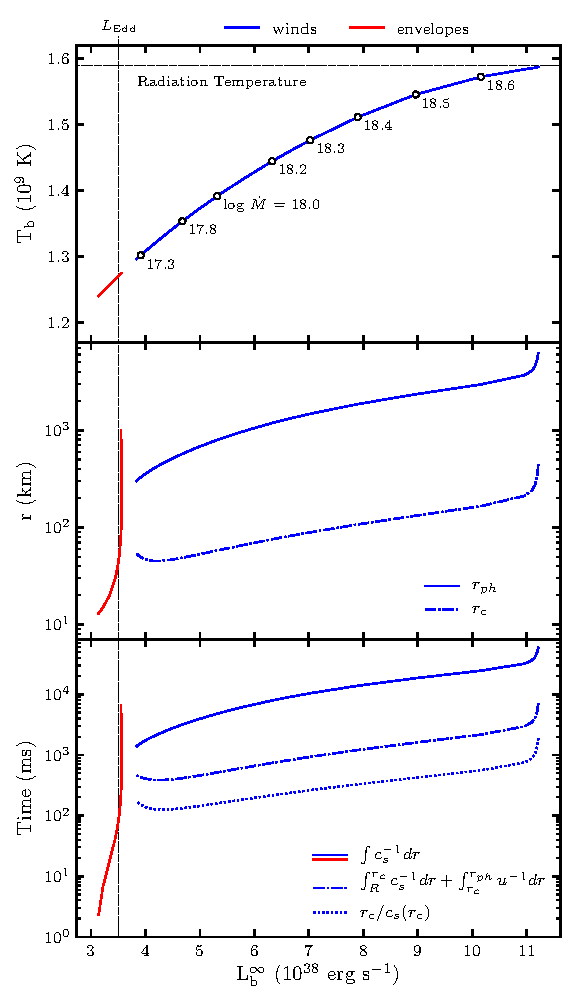
\includegraphics[width=0.7\textwidth]{figures/triple.pdf}
    \caption{Solution space for the base luminosity as seen by observers at infinity, for both winds (blue) and envelopes (red).  Eddington luminosity is marked by the vertical black dashed line. \textit{Top}: Temperature at the base.  Mass-loss rates are indicated at various points for the winds.  \textit{Middle}: Photospheric and critical point radii.  A discontinuity exists between the two regimes (see text).  \textit{Bottom}: Characteristic timescales of the solutions from the base to the photosphere.}
    \label{fig:triple}
\end{figure}

While the static to outflowing transition seems to be smooth when looking at the base, it clearly is not if we study the extended regions, and in particular the photospheric radius (see figure \ref{fig:triple}).  It is therefore not possible to transition from one regime to the other in a quasi-static way, i.e by going from one stationary solution to the other when changing the base flux.  While both regimes may exist for some time if the base flux remains close to constant, the transition can only be modelled by fully time-dependent calculations. 

Furthermore, while these are all analytic solutions to stationary equations, they might not all be stable to small perturbations.  We look at characteristic timescales in the third panel of figure \ref{fig:triple}.  A natural timescale for static structures would be the sound crossing time.  For the winds, we can also take the critical point divided by the sound speed at that time as a relevant timescale, or a dynamic crossing time where we take the flow speed rather than the sound speed in the supersonic region.  In all cases, it is clear that the photospheric radius dictates the timescale, meaning that more extended structures take longer to adjust to small perturbations.  Typical bursts have a rising phase of $\sim1$ s, a super-Eddington or PRE phase of $\sim10$ s and a decaying phase of $\sim1$ min.  Since the rising phase is so fast in transitioning from sub to super-Eddington luminosities, it is clear that our stationary solutions are not appropriate for describing its dynamics.  However, the timescales would allow for PRE and decaying phase to be reasonably be modelled by stationary winds and envelopes respectively, except for the transition from super to sub-Eddington luminosities in the decay.  Finally, the largest static atmospheres with slightly super-Eddington fluxes are unlikely to occur, or at least to remain stable, as their timescales are very long.

\subsection{On the definition of the photosphere}

\biblio
\end{document}
